
\chapter{The "XYZ" Prototype System}
%\index{TODO CHANGE: XYZ}
% NOTES / TODOs:
%
% Architecture scheme, implementation
% callback functions, hot plugin
% js-select selectors
% List of condition operators
% Why JS, why wasnt it used before? is it used now?
% Terminierungsproblem (compiler bau), loesungsansaetze

% Required use cases since their application was promised before in the thesis:
% smart filtering
% aggregation of information in whatever location user wants
% 
The "XYZ" prototype system is the realisation of a reactive web system.
It was developped during the research for this thesis and acts as a platform for feasibility studies of certain use cases.




\section{Architecture}
"XYZ" consists of a queue in which all incoming events are pushed, and an engine that picks the events from the end of the queue whenever it is idle.
Since "XYZ"'s core functionalty is the communication with resources in the web, the architecture bases on HTTP protocol in several parts.
For example the events are meant to be retrieved completely via HTTP, the user interface is a webpage which posts requests to the system and most actions are also meant to be HTTP requests, or at least using them to gather information.

\begin{figure}[!ht]
	\centering
  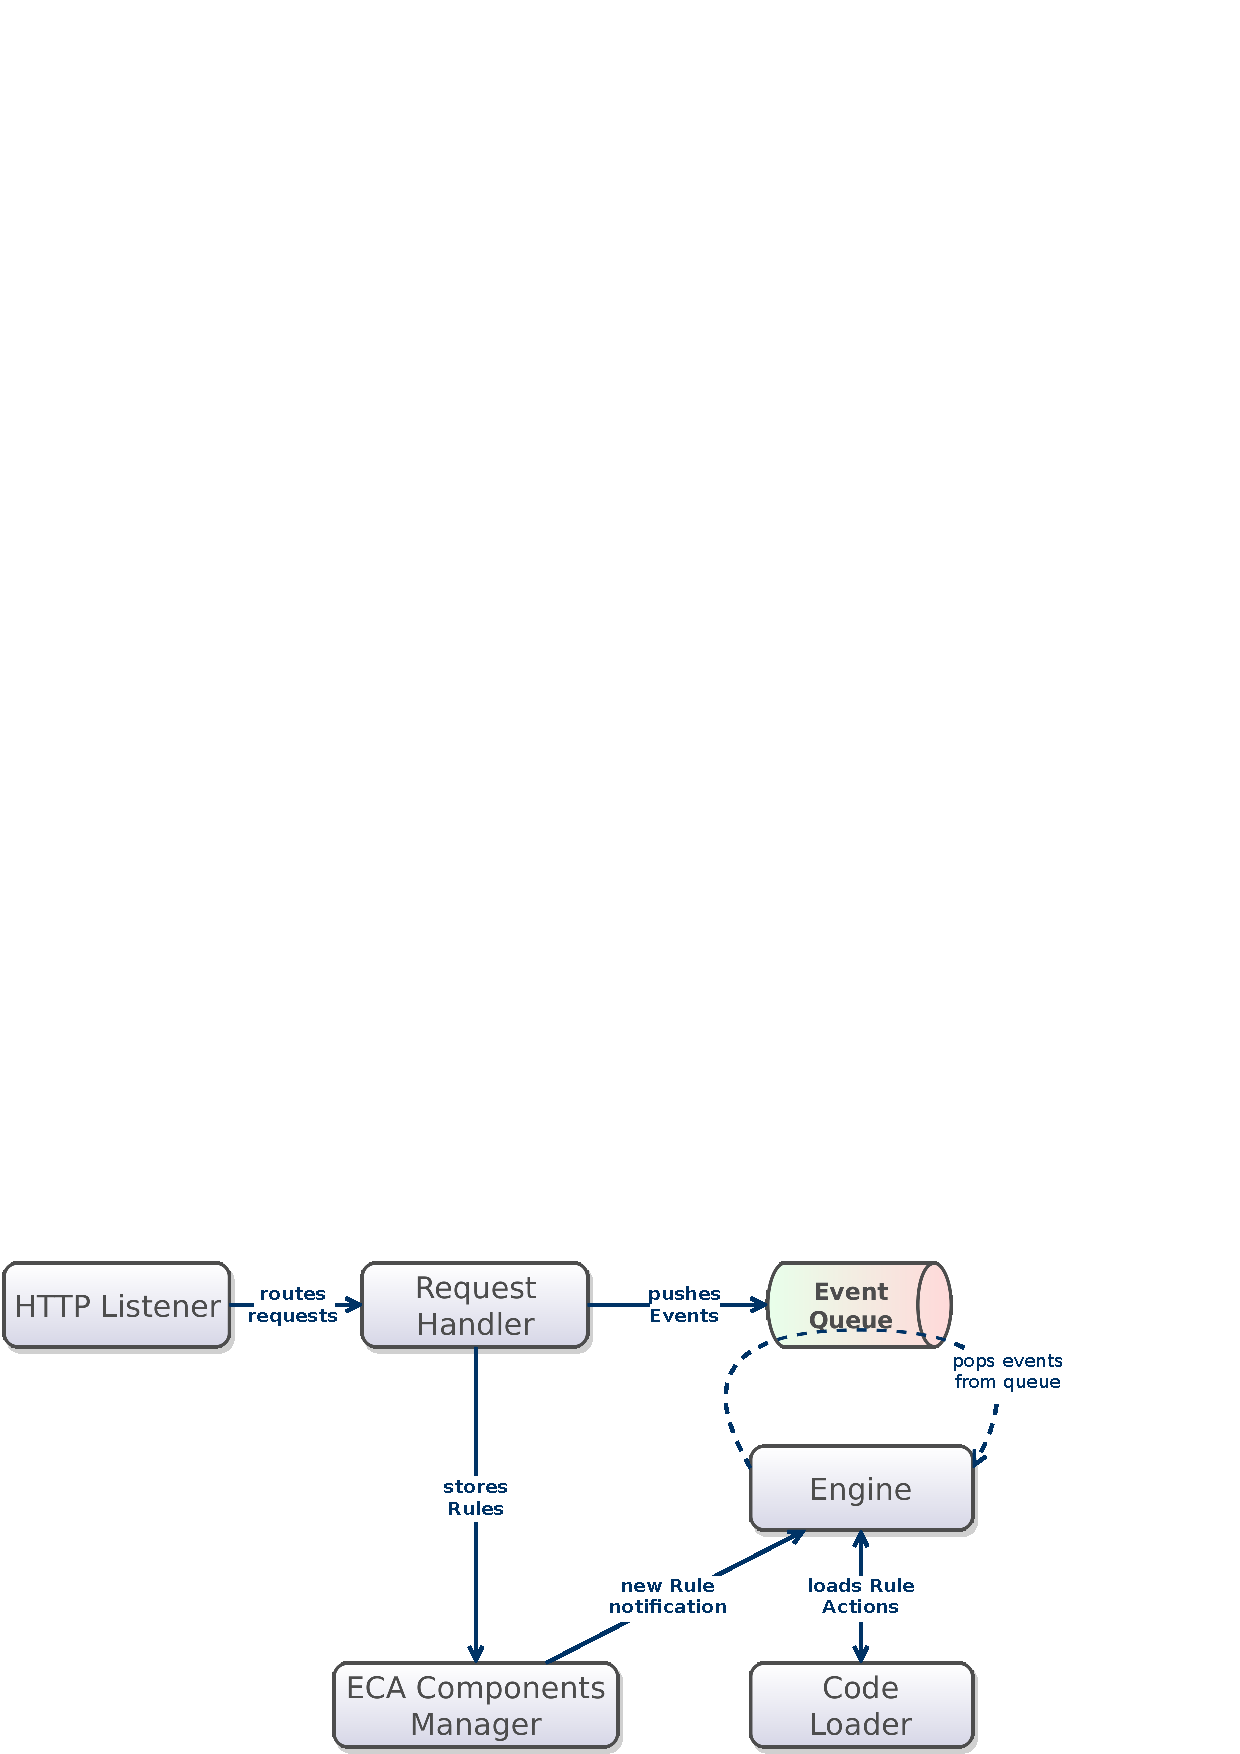
\includegraphics[width=0.8\textwidth]{figures/Architecture_woET}
	\caption{"XYZ" Architecture}
	\label{fig:Architecture_woEP}
\end{figure}

\begin{figure}[!ht]
	\centering
  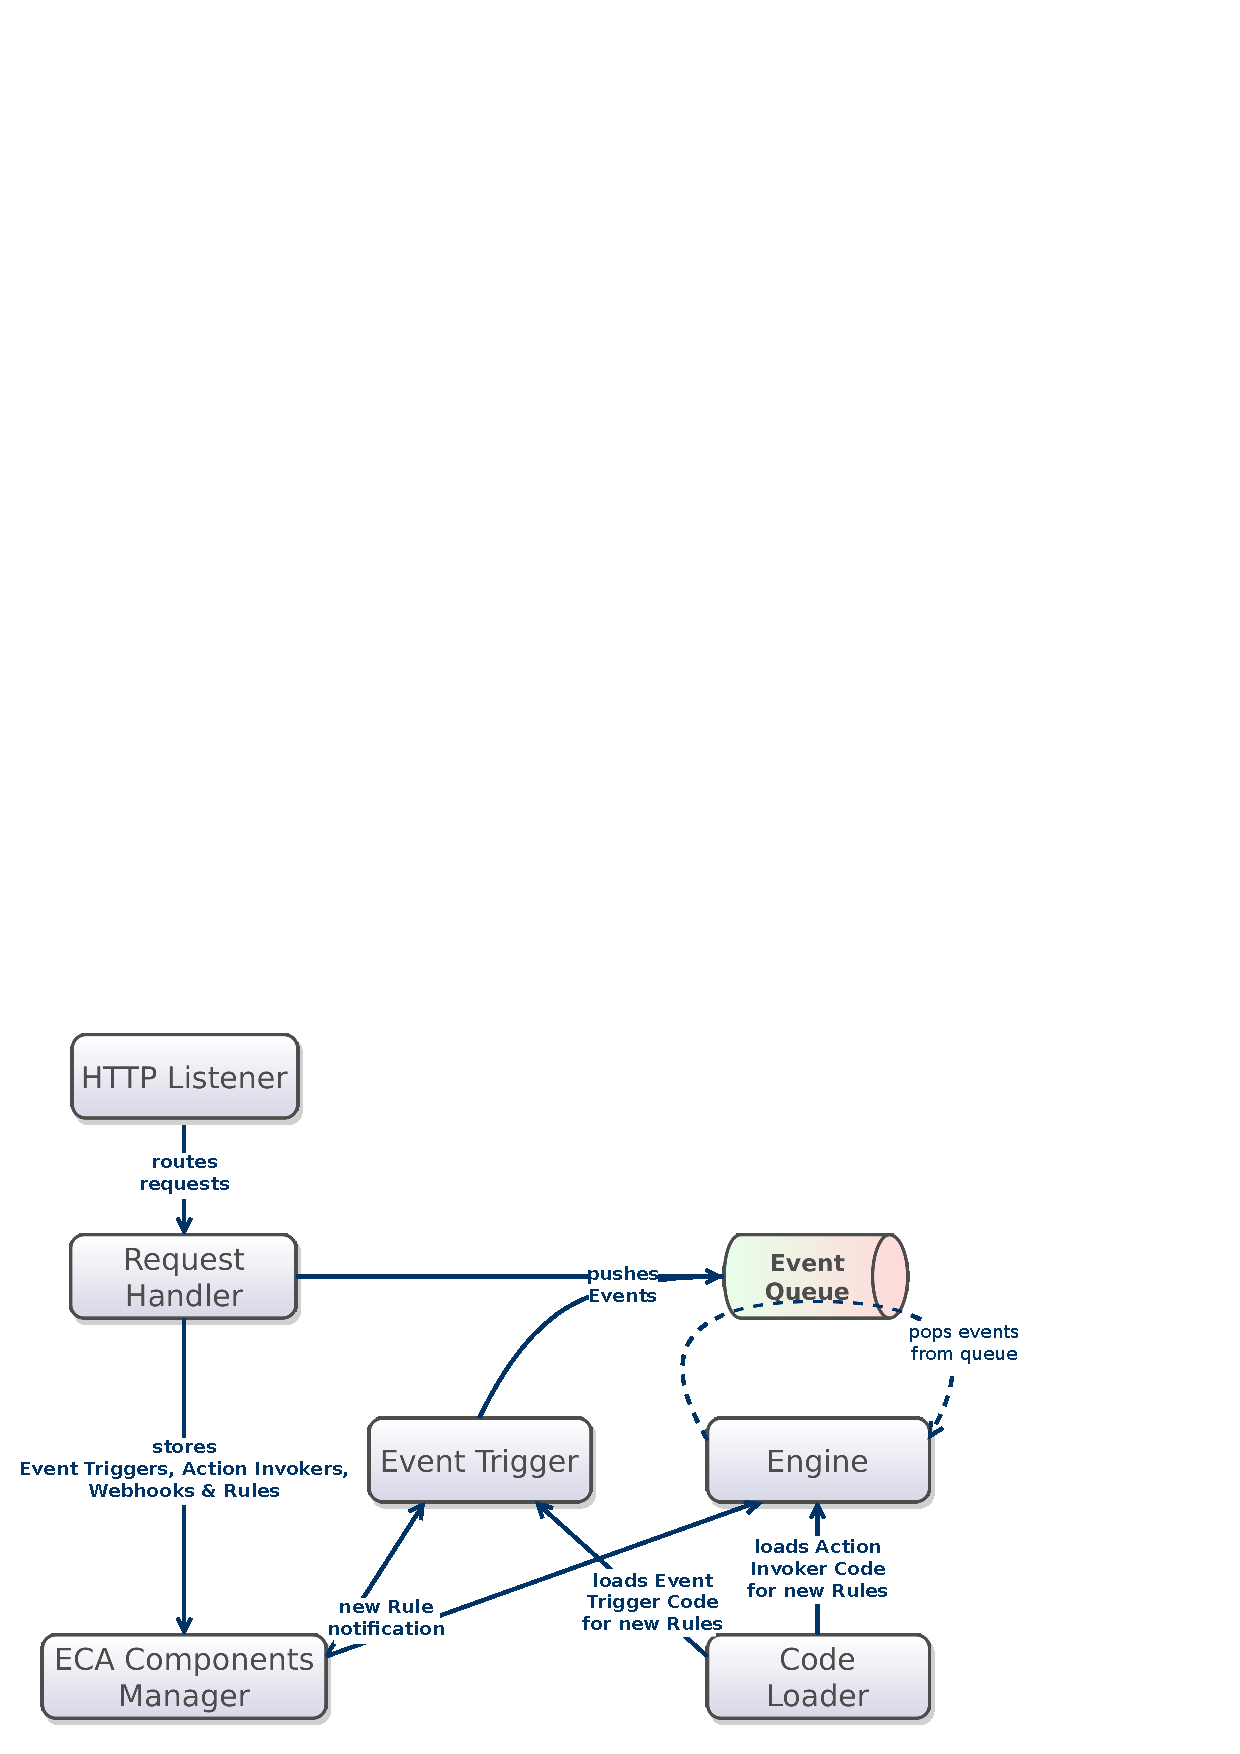
\includegraphics[width=0.9\textwidth]{figures/Architecture_wET}
	\caption{"XYZ" Architecture}
	\label{fig:Architecture_wET}
\end{figure}


\section{Event Triggers}

Event Gathering is the E in ECA and without one of these letters such a system would not run.
It is of utmost importance to find as much as possible ways to get data into a system.



\subsection{Polling}



\subsection{Webhooks}




\section{Conditions}




\section{Actions}

\subsection{Aditional Information}
% Not only from events
% import.io

\section{ECA Rules}





\section{Engine}

% Apply variable number of function arguments to function





\section{Asynchronous Closures}
% NOTES / TODOs:
%
% Variable bindings
% Closures (https://developer.mozilla.org/en-US/docs/Web/JavaScript/Guide/Closures)$
% Closures are functions that refer to independent (free) variables. 
% In other words, the function defined in the closure 'remembers' the environment in which it was created in.

% write about arallel as well?

Often, optimization approaches and programming language concepts require special attention to avoid common pitfalls.
When closures are used as asynchronous functions, developers need to be very careful not to end up with race conditions.


Looking at an example of sequential code execution in Figure~\ref{fig:Closures_Synchronous}, we see that function execution of \texttt{fA} is halted until function \texttt{fB} is finished.
If \texttt{fB} happens to be a latency-driven I/O operation the completion of \texttt{fA} could be deferred for a relatively long time.
While the application waits for the completion of the I/O operation, some remaining operations in \texttt{fA} could eventually already be executed without causing any race conditions.
\begin{figure}[!ht]
	\centering
  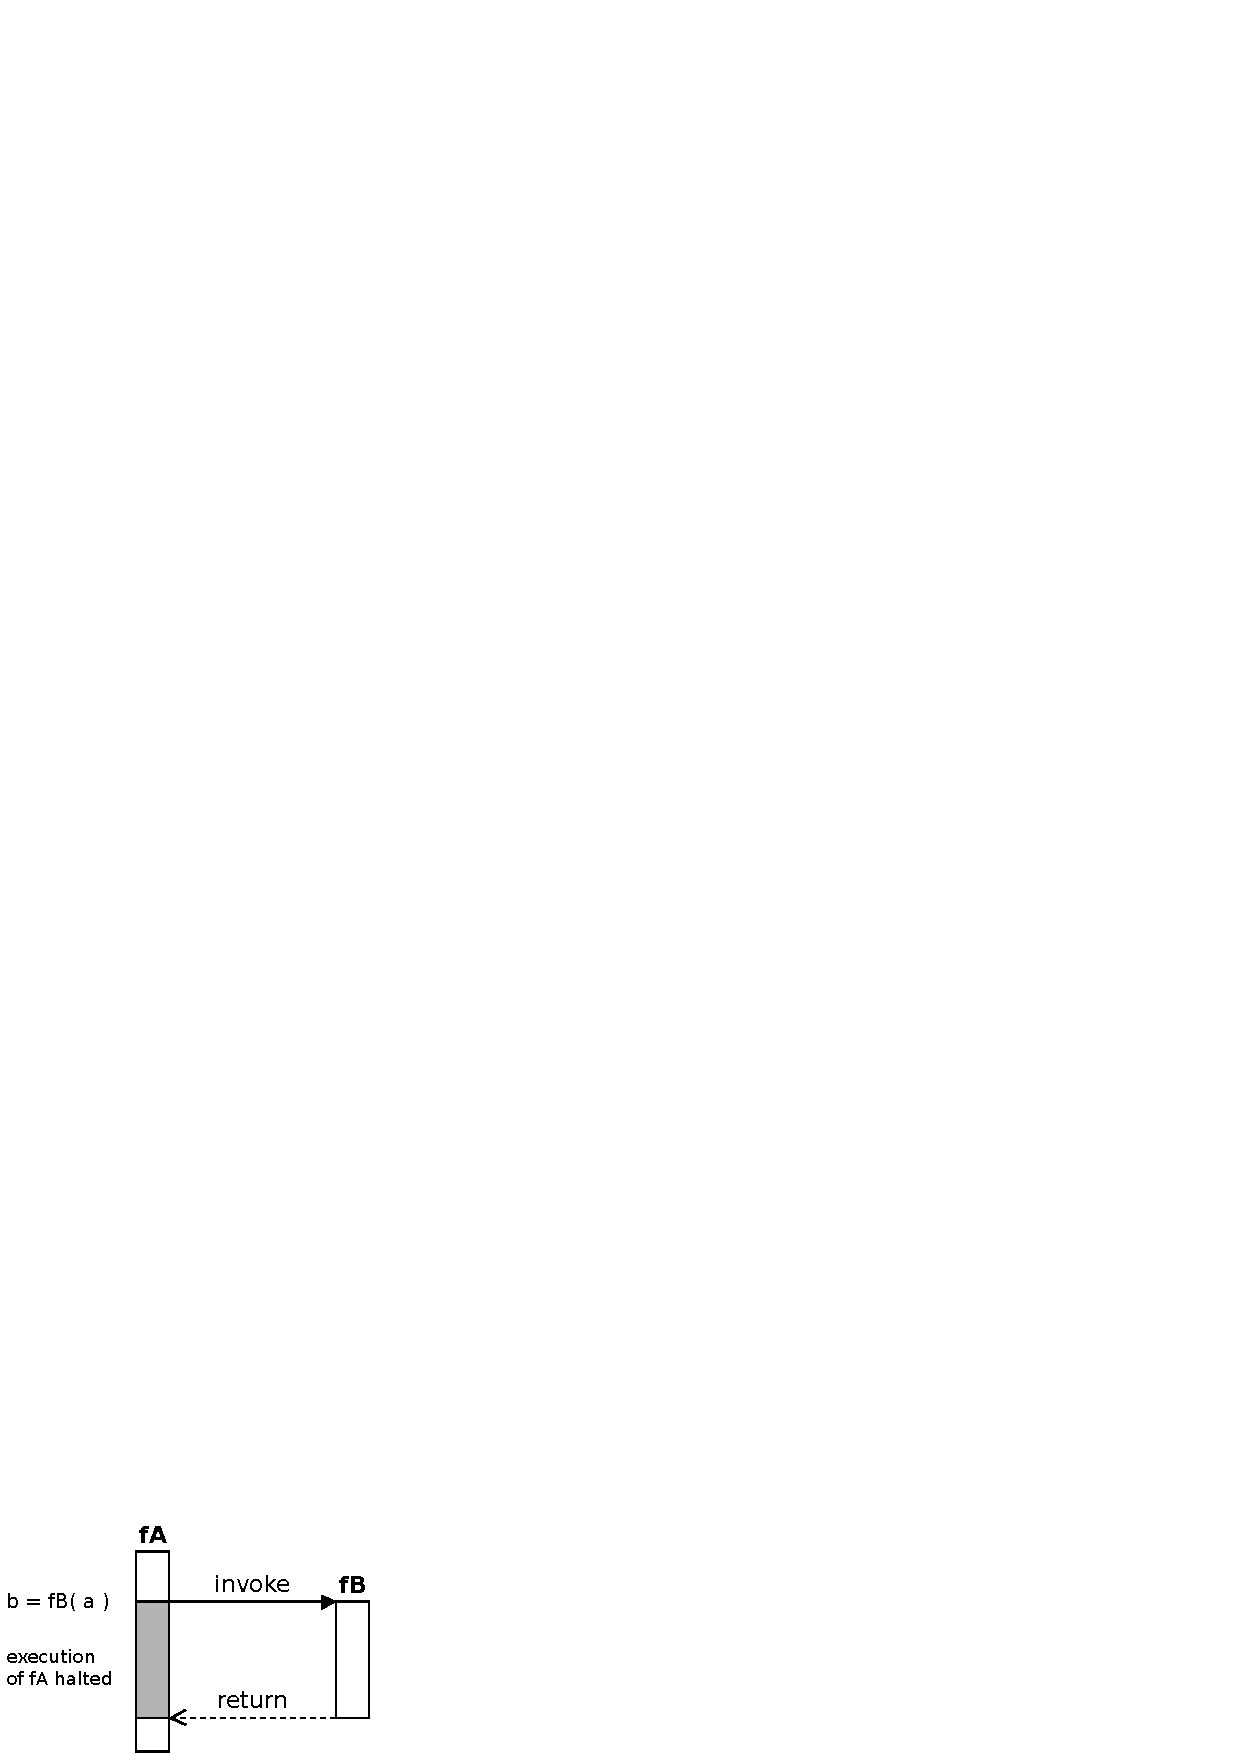
\includegraphics{figures/Closures_Synchronous}
	\caption{Synchronous Function Call}
	\label{fig:Closures_Synchronous}
\end{figure}


Asynchronous code execution, as shown in Figure~\ref{fig:Closures_Asynchronous}, allows non-blocking and thus scalable applications.
Non-blocking operations are a remedy for optimzed resource allocation and open up ways to overcome previously described unnecessary resource bindings.
Processing any kind of latency-driven I/O operation asynchronously ( e.g. filesystem access and socket communication ) exploits resources that would otherwise be bound while waiting for completion.
Such operations are processed and completed whenever required resources are available.
\begin{figure}[!ht]
	\centering
  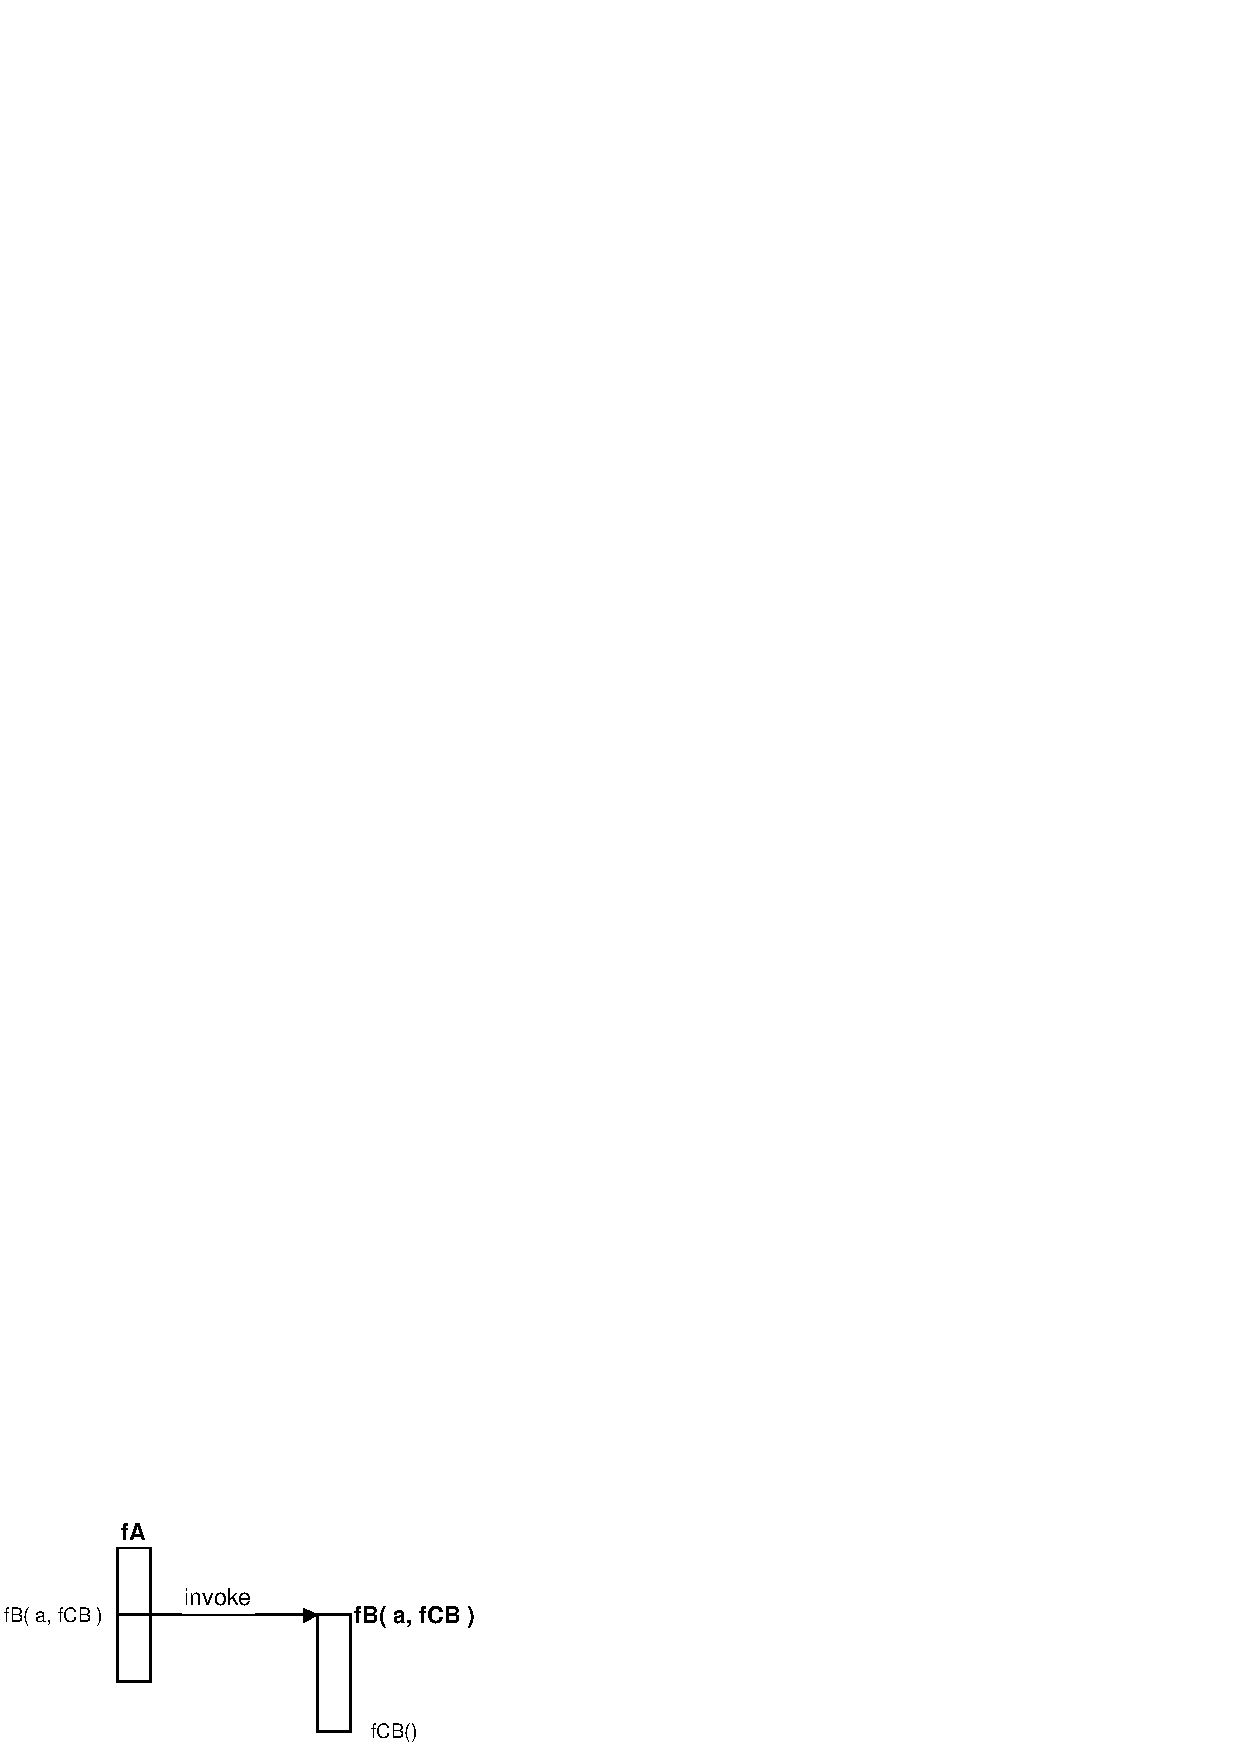
\includegraphics{figures/Closures_Asynchronous}
	\caption{Asynchronous Function Call}
	\label{fig:Closures_Asynchronous}
\end{figure}


Often other operations depend on the completion of asynchronous operations, hence their execution needs to be deferred.
This necessary code execution deferral is achieved through the use of callback functions, denoted \texttt{fCB} in Figure~\ref{fig:Closures_Asynchronous}.
Any code placed in a callback function, which is assigned to an asynchronous operation, is only executed after the respective asynchronous operation completed.
This allows stacking of functions and operations upon each other which automatically results in a flexible and event-driven application.


Now we take closures into this asynchronous context, as defined in ECMAScript\cite{EcmaScript}, which is the base for widely-spread script languages like JavaScript, JScript and ActionScript.
Closures in ECMAScript\cite{EcmaScript} are defined such as they have access to the context of the function they were created in.
This is shown in Figure~\ref{fig:Closures_Closure-1} where \texttt{c} from \texttt{fA}'s context is accessible from within \texttt{fB}, assuming that \texttt{fB} was created in \texttt{fA} and not only invoked from there.
Using asynchronous closures it becomes evident, that the context in the invoking function can change while the closure is still computing and eventually referencing the outer context, thus causing race conditions.
This will be most obvious in a loop that immediately invokes \texttt{fB} several times, as shown in Figure~\ref{fig:Closures_Closure-2}.
In such a setup \texttt{c} will have different values in the same part of different invocations of \texttt{fB}.
This might be a very well hidden pitfall since often developers will take care that the context will not change during execution of \texttt{fA}.
But it is likely that the context will change if \texttt{fA} is invoked again while \texttt{fB} is still running, which is a common behaviour in event-driven architectures.
\begin{figure}[!ht]
	\centering
  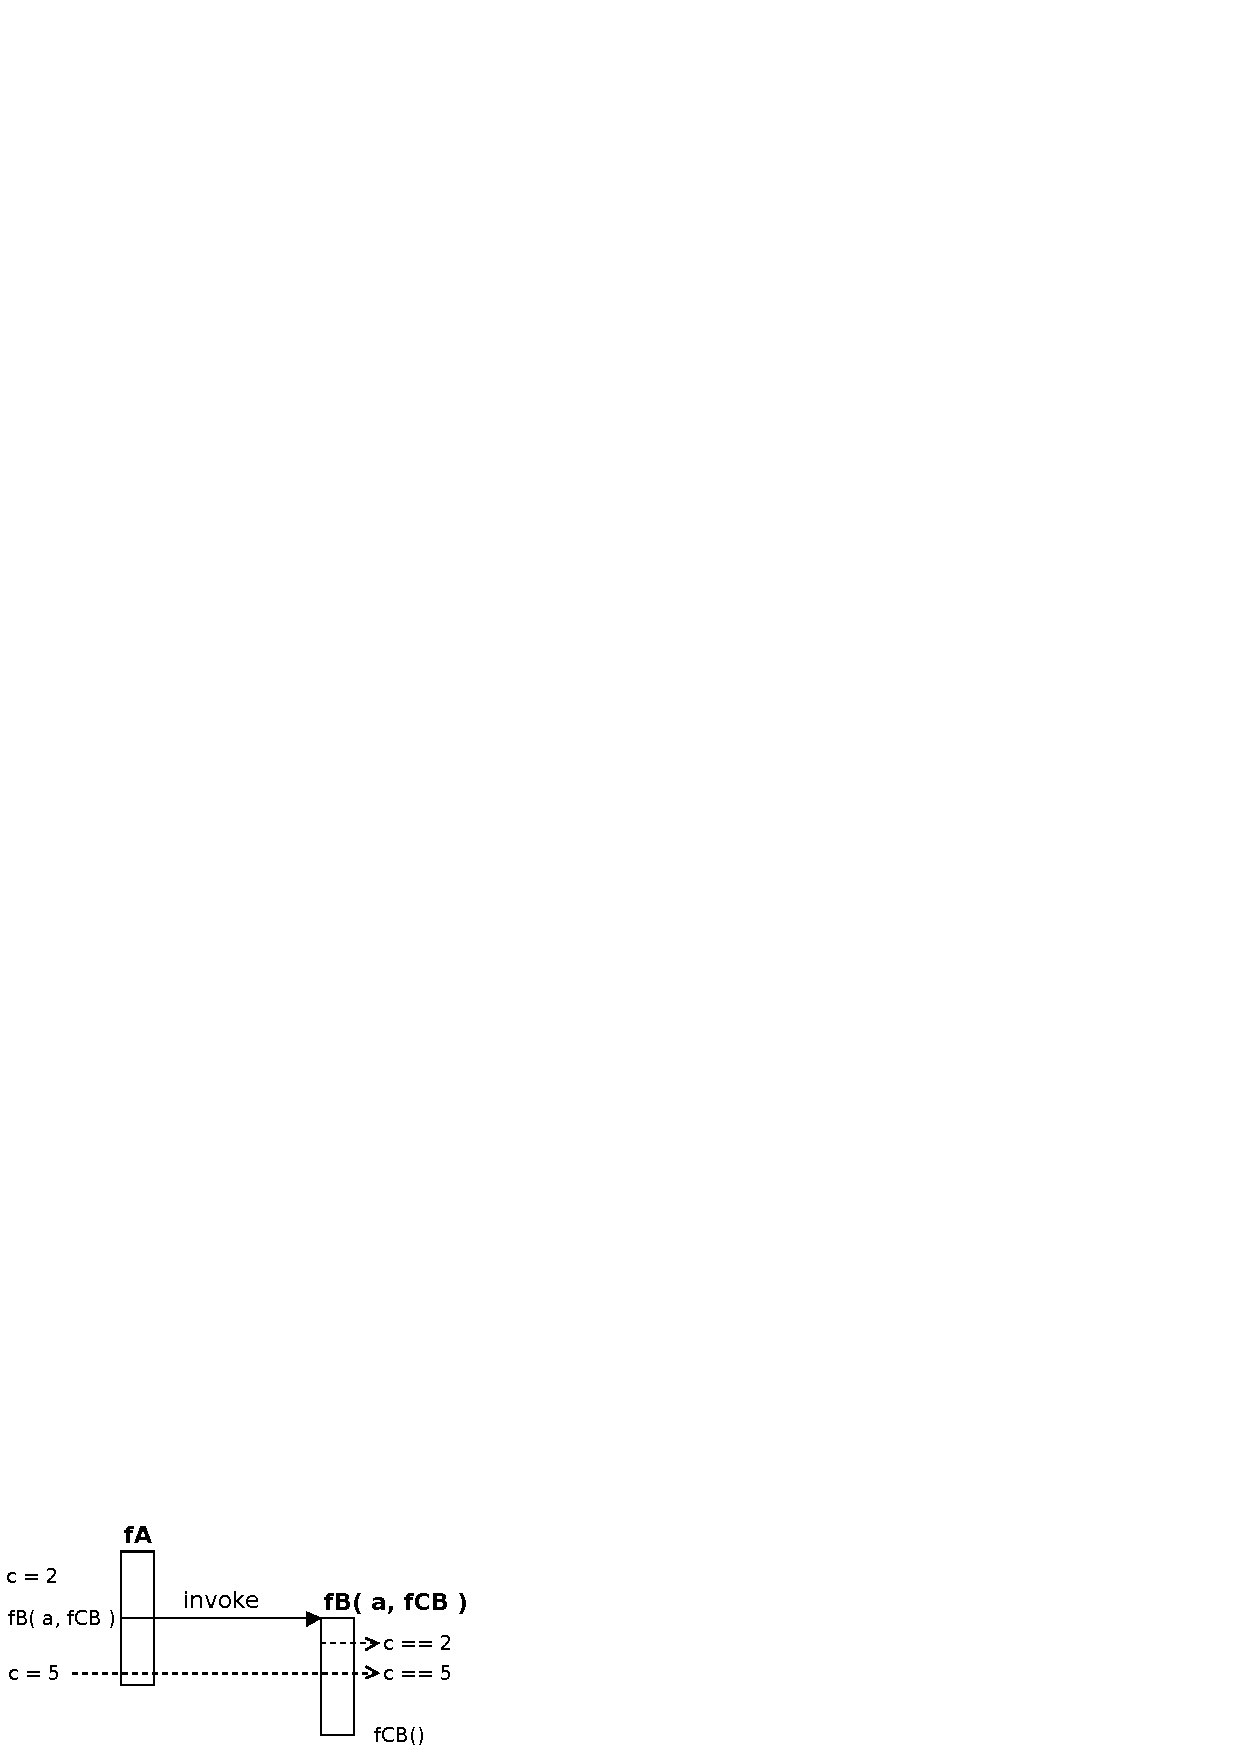
\includegraphics{figures/Closures_Closure-1}
	\caption{Closure Scope and referenced context}
	\label{fig:Closures_Closure-1}
\end{figure}
\begin{figure}[!ht]
	\centering
  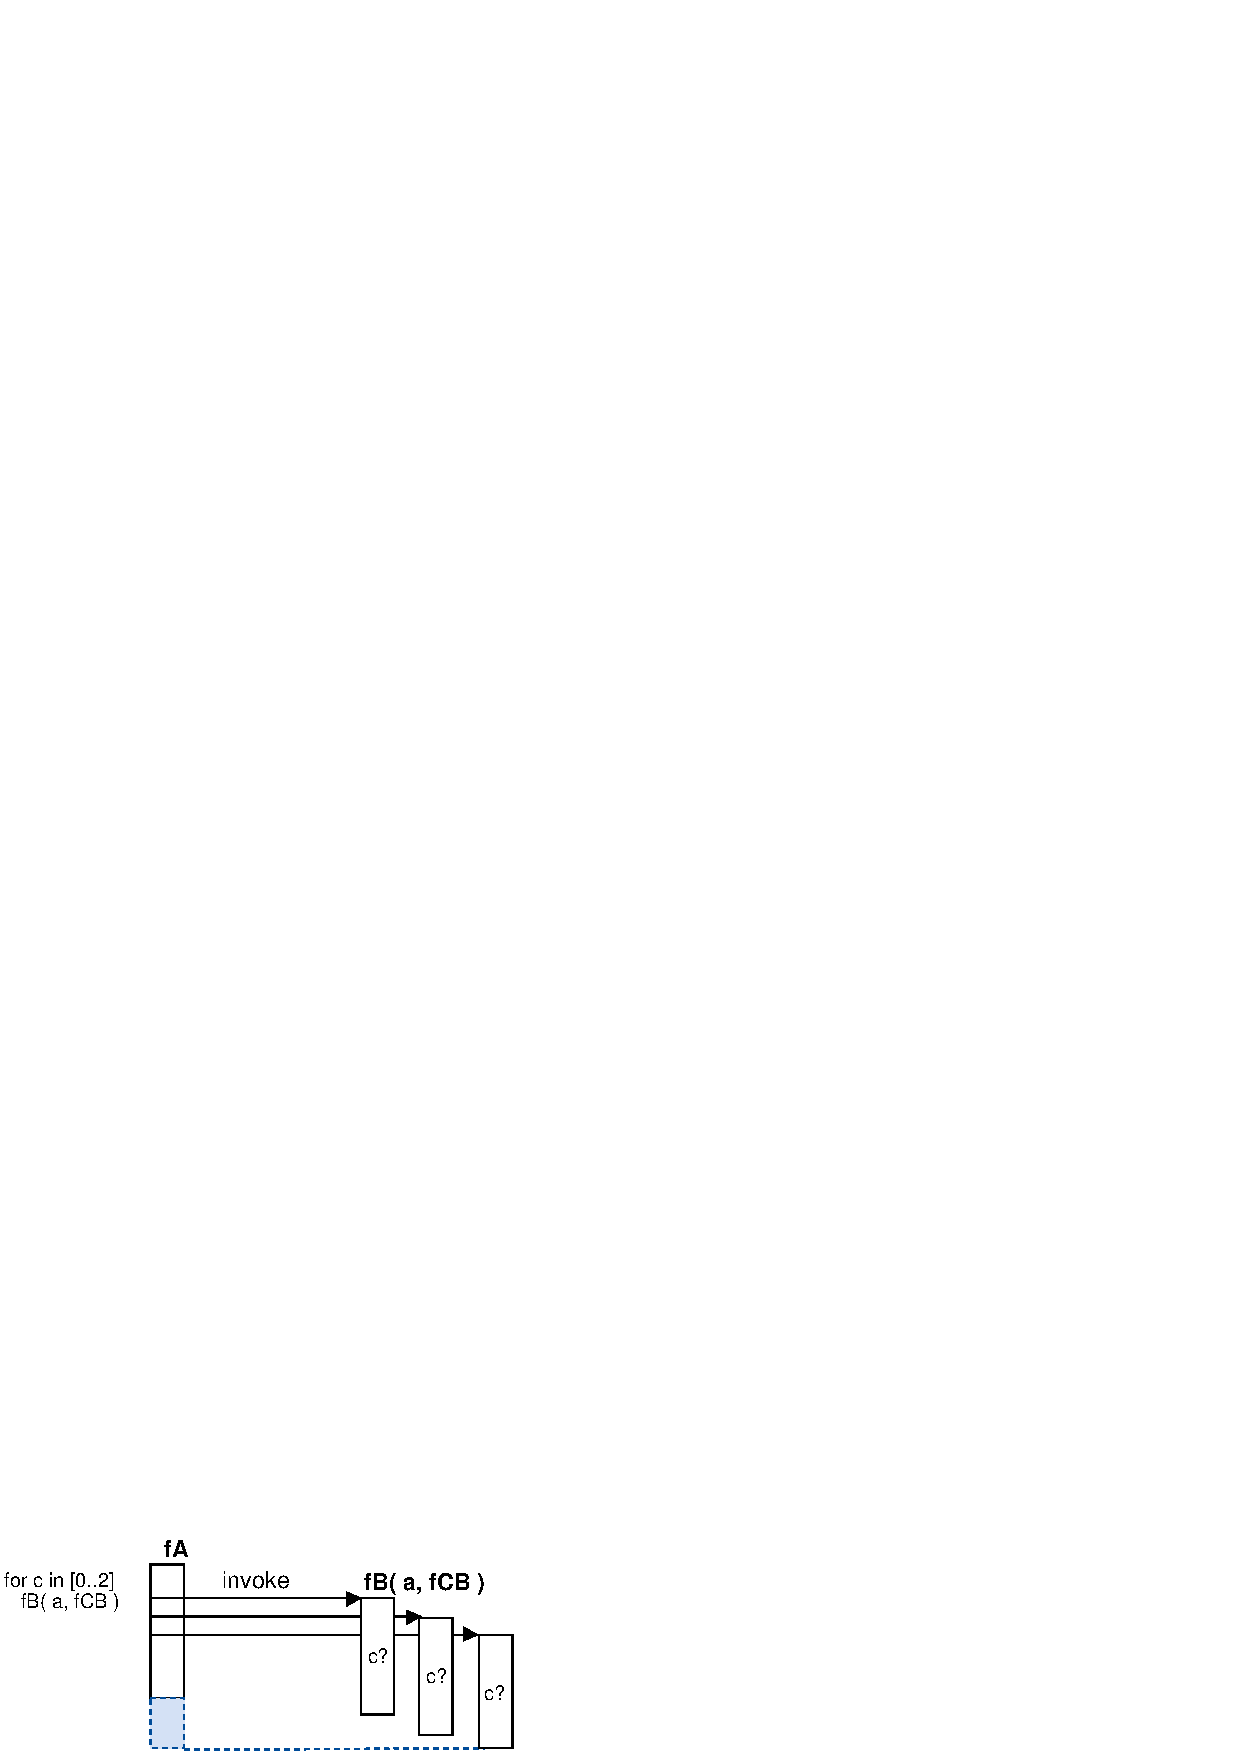
\includegraphics{figures/Closures_Closure-2}
	\caption{Closure context changes in a loop}
	\label{fig:Closures_Closure-2}
\end{figure}


Those event-driven context overwrites can be taken care of by shielding the closure from context changes, as shown in Figure~\ref{fig:Closures_Closure-3}.
To shield the closure form context changes, closure \texttt{fB} needs to create another closure \texttt{fC} and return it to \texttt{fA}.
The argument passed to \texttt{fB} is the context ( \texttt{c} in Figure~\ref{fig:Closures_Closure-3} ) that might change but requires to be persistent for one invocation.
\texttt{fC} has now \texttt{c} as a fixed context, which can't be overwritten anymore.
Now the only thing left is \texttt{fC} needs to be invoked and it will retain the original context.
This implementation is necessary when the closure acts as a callback function for asynchronous operations, to preserve the original context in case it is required within the callback function.
\begin{figure}[!ht]
	\centering
  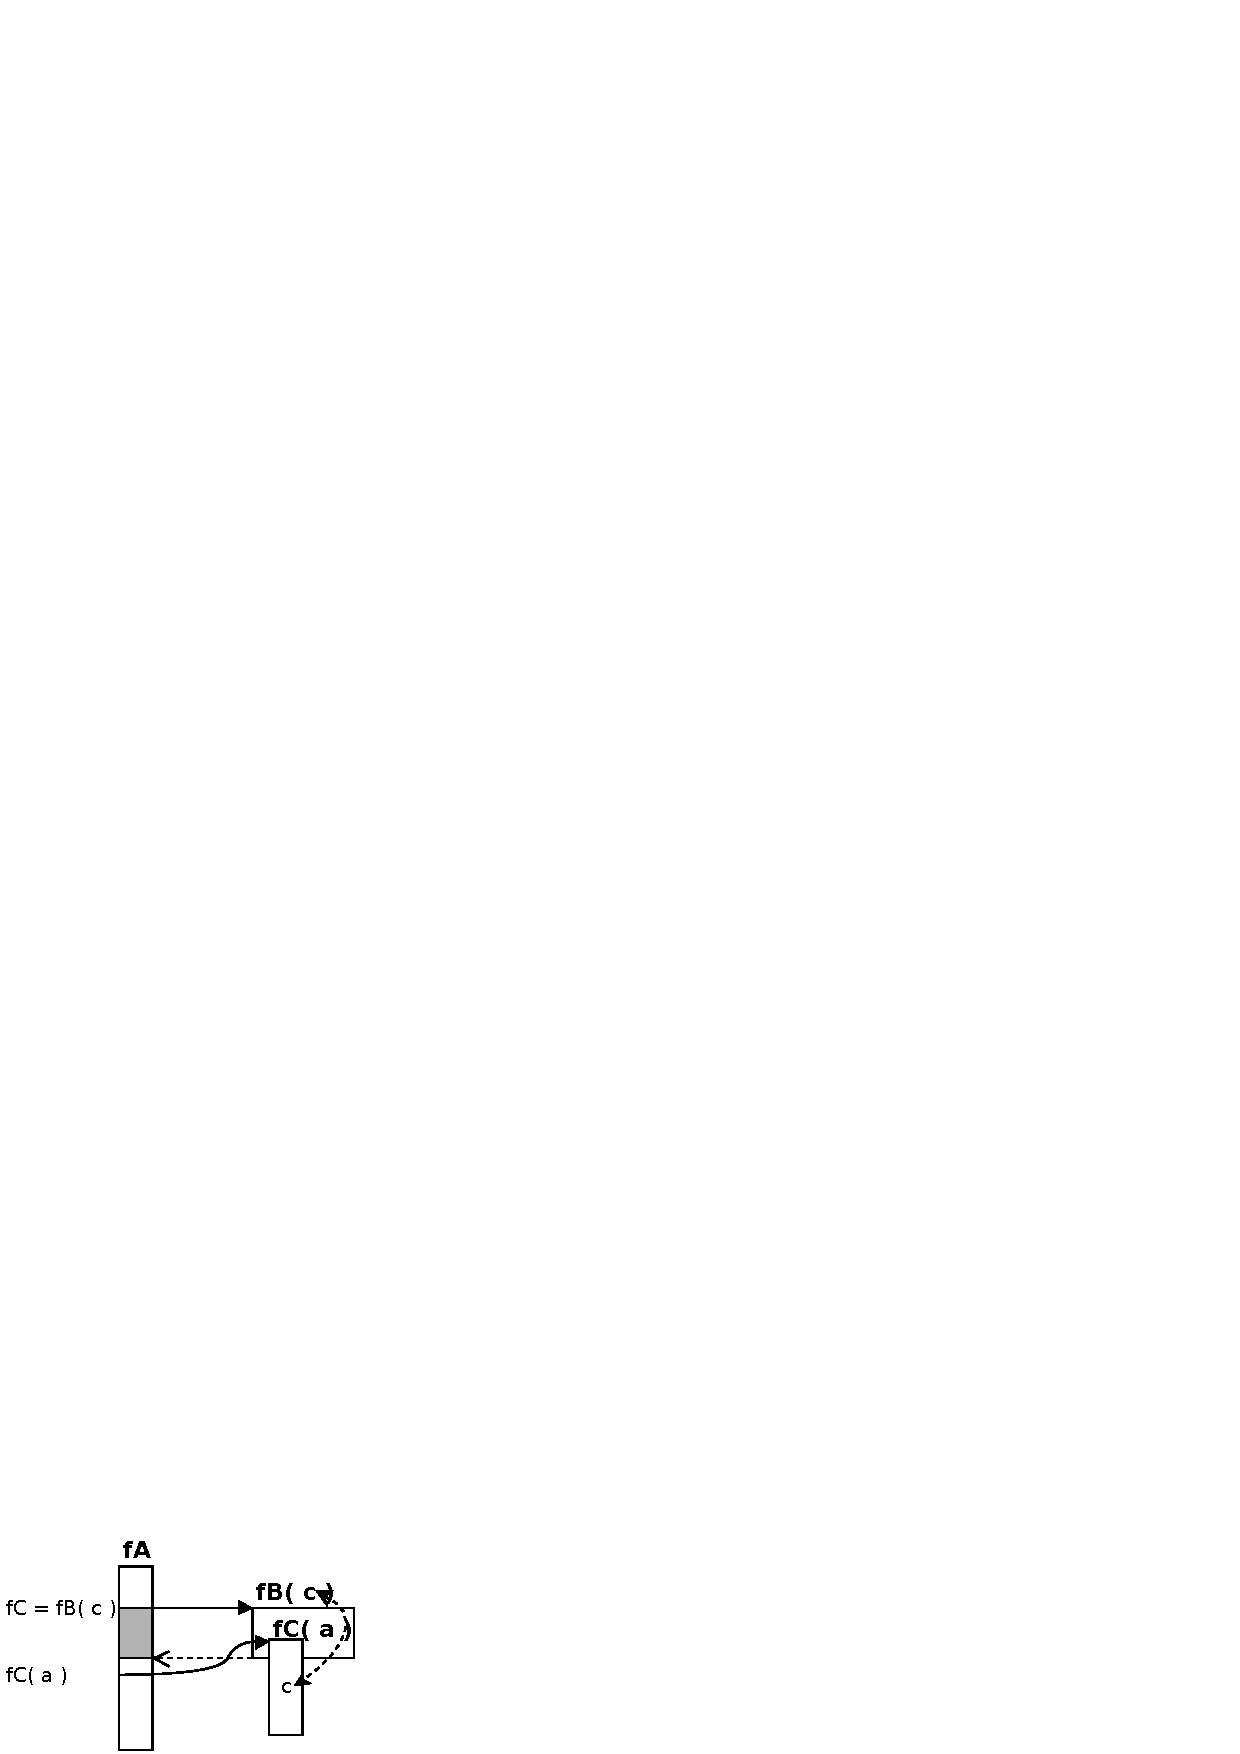
\includegraphics{figures/Closures_Closure-3}
	\caption{Closure context shielding}
	\label{fig:Closures_Closure-3}
\end{figure}

% TODO try async closures in other programming languages


\section{Node.js}

\subsection{Benchmarking JavaScript vs. Java}

\begin{lstlisting}[frame=single,label=lst_bm_java,language=Java,caption=Closure Benchmarking: Java Code]
/*
 * BenchmarkingDeferred.java
 */
import java.util.concurrent.ScheduledExecutorService;
import java.util.concurrent.Executors;
import java.util.concurrent.TimeUnit;
import java.util.HashMap;

public class BenchmarkingDeferred {

  private static Runtime runtime = Runtime.getRuntime();
	private static final ScheduledExecutorService worker = 
		Executors.newSingleThreadScheduledExecutor();

	private static void deferFunctionCall( int numScopeVars, int delay, String scopeId ) {
		HashMap<String, String> mapVars = new HashMap<String, String>();
		for( int i = 0; i < numScopeVars; i++ ) {
			mapVars.put( "id" + i, "12345678" ); // 8 bytes per stored scope variable
		}
		Object context = new TimeoutContext( "TimeoutFunction" );
		Runnable task = new RunnableCallbackFunction( mapVars, context );
		worker.schedule( task, delay, TimeUnit.SECONDS );
	}

	public static void main( String[] args ) {
		long startTime, stopTime;
		int numVars = 10, firstArg = 0;
		firstArg = Integer.parseInt( args[0] );
		numVars = Integer.parseInt( args[1] );
		int j = 0, numFuncs = 1 << firstArg;

		startTime = System.nanoTime();
		while( j++ < numFuncs) {
			deferFunctionCall( numVars, numFuncs * 10, numFuncs + "(" + j + ")" );
		}
		stopTime = System.nanoTime();

		// [...] benchmark system out

		worker.shutdownNow();
	}
}

/*
 * RunnableCallbackFunction.java
 */
import java.util.HashMap;

/*
 * The Callback function instance.
 */
public class RunnableCallbackFunction implements Runnable {
	
	// The hashhmap is used to store variables and their value as the scope
	private HashMap<String, String> mapScope;
	private Object context;

	public RunnableCallbackFunction( HashMap<String, String> scope, Object context ) {
		this.mapScope = scope;
		this.context = context;
	}

	// If this is executing, we didn't wait long enough and the
	// benchmark time is compromised
	public void run() {
		System.out.println( mapScope.toString() );
	}

}

/*
 * TimeoutContext.java
 */
public class TimeoutContext {
	private long idleTimeout = 1;
  private long idlePrev;
  private long idleNext;
  private long idleStart = 140000505;
  private String onTimeout = null;
  private boolean repeat = false;

	public TimeoutContext( String cb ) {
		this.onTimeout = cb;
	}
}

\end{lstlisting}

\begin{lstlisting}[frame=single,float=h,label=lst_bm_js,language=JavaScript,caption=Closure Benchmarking: JavaScript Code]
/*
The function deferral measurements in node.js
*/

var deferredFunction = function ( numScopeVars, delay, scopeId ) {
	var scope = {};
	for ( var i = 0; i < numScopeVars; i++ ) {
		scope[ "id" + i ] = "12345678"; // 8 bytes per stored scope variable
	}
	setTimeout( function () {
		// If this is executed we didn't wait long enough
		console.log( JSON.stringify( scope, null, '  ' ) );
	}, delay );
}

var numOfFunctions,
		numOfScopeVars = process.argv[ 3 ];

numOfFunctions = Math.pow( 2,  process.argv[ 2 ] );

var time = process.hrtime();
for (var i = 0; i < numOfFunctions; i++) {
	deferredFunction( numOfScopeVars, 1000 * numOfFunctions, numOfFunctions + "(" + i + ")" );
};
var diff = process.hrtime( time );

var mem = process.memoryUsage();
// [...] benchmark system out
process.exit( 0 );

\end{lstlisting}


\newpage
{\huge "XYZ" Name discussion}
% WECAST

% WebAPI
% ECA
% Engine
% Reactive
% Web
% Demo
% WebAPI
% System
% Services
% Multipurpose 
% Prototype
% Kernel
% General-Purpose
% Programmable
% Programmable Web 


% General-Purpose ECA Engine Kernel
\textbf{Examples for XYZ:}
\begin{itemize}
  \item \textbf{GEEK} (General-Purpose ECA Engine Kernel)
  \item \textbf{DECADE} (Dynamic ECA Demo Engine)
  \item \textbf{WECAST} (WebAPI ECA Service Trigger)
  \item \textbf{RECAST} (Reactive ECA Service Trigger)
  \item \textbf{PECAN} (Productive ECA eNgine)
  \item \textbf{ICECAP} (Inet-Service Calls through ECA Paradigm)
\end{itemize}
